\usetikzlibrary{arrows.meta,calc}
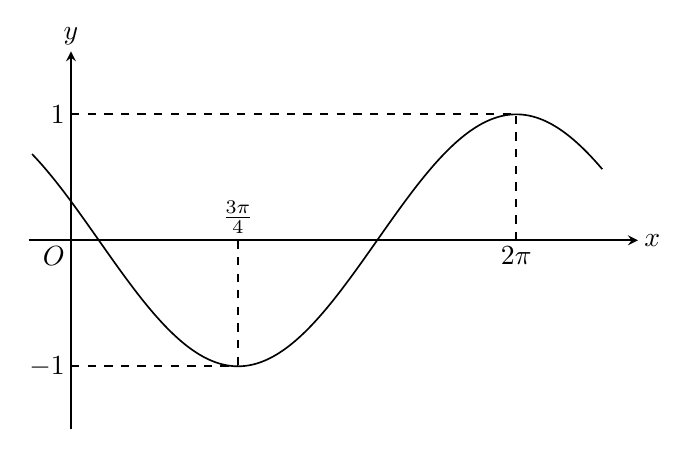
\begin{tikzpicture}[x=0.9cm,y=1.6cm,line width=.6pt,>=stealth,font=\normalsize]
\draw[->] (-0.6,0) -- (8.0,0) node[right,inner sep=0pt,xshift=2pt] {$x$};
\draw[->] (0,-1.5) -- (0,1.5) node[above,inner sep=0pt,yshift=2pt] {$y$};
\node[below left,inner sep=0pt,xshift=-2pt,yshift=-2pt] at (0,0) {$O$};
\draw[dashed] (0,1) -- (6.2831853,1);
\draw[dashed] (0,-1) -- (2.3561945,-1);
\draw[dashed] (2.3561945,0) -- (2.3561945,-1);
\draw[dashed] (6.2831853,0) -- (6.2831853,1);
\draw[domain=-0.55:7.5,samples=220] plot (\x,{sin(deg(0.8*\x)+162)});
\node[left,inner sep=0pt,xshift=-2pt] at (0,1) {$1$};
\node[left,inner sep=0pt,xshift=-2pt] at (0,-1) {$-1$};
\node[above,inner sep=0pt,yshift=2pt] at (2.3561945,0) {$\frac{3\pi}{4}$};
\node[below,inner sep=0pt,yshift=-2pt] at (6.2831853,0) {$2\pi$};
\end{tikzpicture}
